

 Consider the function $$f(x_1,x_2)=50x_1^2-x_2^3$$ illustrated in the figure below.

\begin{center}
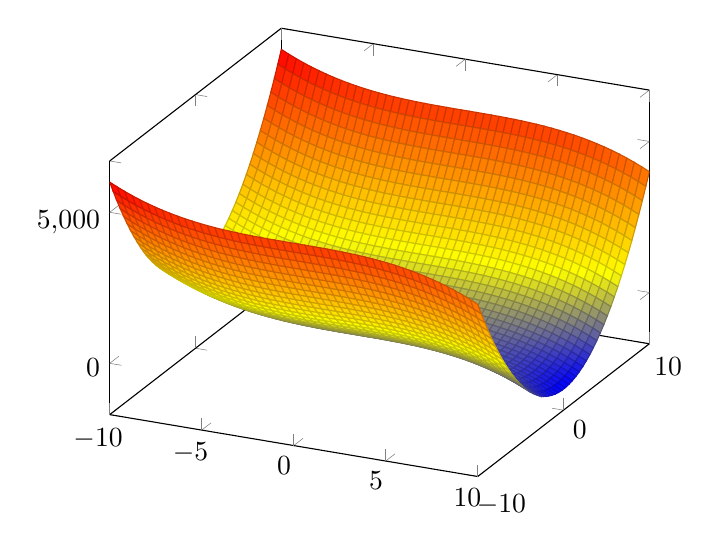
\begin{tikzpicture}
\begin{axis}
\addplot3[surf,domain=-10:10,samples=50]
{50*y^2-x^3};
\end{axis}
\end{tikzpicture}
\end{center} 

\begin{enumerate}
\item Show that the point
  \[
  x^* =  \cvect{0 \\ 0}
  \]
  satisfies the necessary optimality conditions.

\item Show that this point is neither a local minimum nor a local maximum. 
  \textit{Hint: Consider the directions}
\[
    d_1=\cvect{0 \\ 1} \text{ and } d_2=\cvect{0 \\ -1}.
\]
\end{enumerate}


